%%%%%%%%%%%%%%%%%%%%%%%%%%%%%%%%%%%%%%%%%%%%%%%%%%%%%%%%%%%%%%%%%%%
%%% Documento LaTeX 																						%%%
%%%%%%%%%%%%%%%%%%%%%%%%%%%%%%%%%%%%%%%%%%%%%%%%%%%%%%%%%%%%%%%%%%%
% Título:		Introducción
% Autor:  	Ignacio Moreno Doblas
% Fecha:  	2014-02-01, actualizado 2019-11-11
% Versión:	0.5.0
%%%%%%%%%%%%%%%%%%%%%%%%%%%%%%%%%%%%%%%%%%%%%%%%%%%%%%%%%%%%%%%%%%%
% !TEX root = A0.MiTFG.tex

\chapterbegin{Introducción y visión general}
\minitoc

\section{Problemática de los accidentes de tráfico}

Cada año en el mundo la vida de, aproximadamente, 1.35 millones de personas termina por culpa de accidentes de tráfico. Además, entre 20 y 50 millones de personas más sufren lesiones no mortales y muchas de ellas padecen una discapacidad a causa del accidente. \cite{who1}

Estas cifras son extremadamente altas y lo más preocupante es que constituyen la principal causa de muerte entre los jóvenes de 15 a 29 años. Alrededor del 73\% de todas las defunciones por accidentes de tránsito afectan a hombres menores de 25 años. A su vez, las personas de entre 15 y 44 años representan el 48\% de las defunciones por accidentes de tráfico en todo el mundo. \cite{who1}

A lo largo de los años muchas organizaciones han trabajado para mejorar esta situación y aunque en países de ingresos altos como la mayoría de los europeos se ha conseguido descender levemente el número de muertes (no de accidentes) en otros países de ingresos bajos y medianos no se ha logrado y en los últimos 15 años la tasa de muerte por 100 mil habitantes se ha visto muy poco reducida.

Al margen del coste en vidas hay que destacar que los accidentes de tráfico causan pérdidas económicas tanto para los propios individuos, sus familias e incluso los países. Además, muchos familiares necesitan tiempo para recuperarse por el trauma psicológico. Se estima que los accidentes de tráfico suponen una pérdida del 3\% del producto interior bruto de cada país. \cite{who1}

Los factores de riesgo más importantes para que ocurran accidentes son:
\begin{itemize}
    \item Error humano: siempre hay que tener en cuenta la posibilidad del error humano por lo que los sistemas de prevención se deberían desarrollar para tolerar dicho error. Por ello, es importante tener una infraestructura adecuada y segura, así como hacer que los vehículos sean más inteligentes y puedan comunicarse con su alrededor a través de la luz visible.
    \item Velocidad: el aumento de la velocidad está claramente ligado a la mortalidad y gravedad de los accidentes.
    \item Conducir bajo los efectos del alcohol o drogas.
\end{itemize}

En la figura \ref{muertes} se representa la evolución de las muertes por accidentes de tráfico en los 
últimos años en la que se demuestra la leve reducción de la tasa de muertes en los últimos 
años. Por su parte, la figura \ref{distribucion} muestra las muertes en función del usuario
en carretera en la que destaca que los mayores afectados en Europa, América y África son 
los usuarios de vehículos de cuatro ruedas y en Asia y Oceanía son los usuarios de vehículos 
de dos o tres ruedas, siendo las muertes de peatones un elevado porcentaje en todos los 
sitios. \cite{who2}

\begin{figure}[ht]
    \centering
    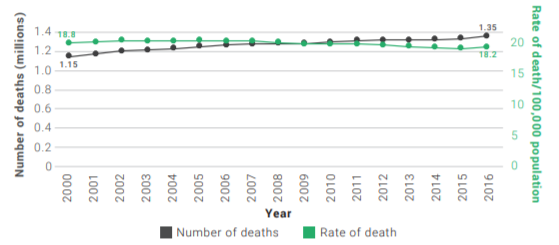
\includegraphics[scale=0.85]{./figuras/muertes_accidentes.png}
    \caption{\small{Número y tasa de muertes por accidentes de tráfico por 100 mil habitantes. Fuente: [2] }}
    \label{muertes}%
\end{figure}

\begin{figure}[h]
    \centering
    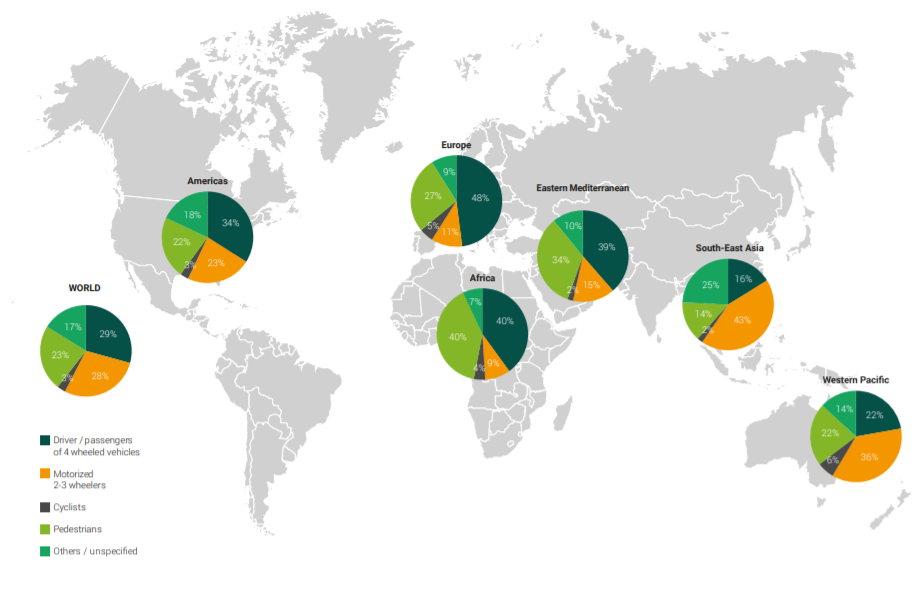
\includegraphics[scale=0.575]{./figuras/distribucion.png}
    \caption{\small{Distribución de muertes por tipos de usuarios en las carreteras. Fuente: [2] }}
    \label{distribucion}%
\end{figure}

\newpage
Este trabajo se centra en el uso de la comunicación mediante luz visible en aplicaciones de automoción para mejorar la seguridad y la protección de las personas. Dicha comunicación se produciría de manera inalámbrica entre vehículos y también con la infraestructura. Gracias a esto la seguridad y la eficiencia del transporte pueden aumentarse sustancialmente para salvar más vidas.
\newpage
\section{Problemática de las ondas electromagnéticas}

El consumo de electricidad ha pasado a formar parte de la vida cotidiana. Ligado a la electricidad se encuentra el campo eléctrico y magnético. Además, hoy en día no se concibe la vida sin las comunicaciones a distancia, desarrolladas gracias a la continua emisión de ondas electromagnéticas. Es cierto que es difícil exponerse a niveles elevados de radiación. En este sentido ha quedado establecido a través de investigaciones científicas que la exposición aguda a niveles elevados, tienen efectos adversos a la salud como estimulaciones neuronales y musculares. También se están estudiando los posibles efectos a largo plazo y aunque no hay ningún estudio concluyente hay indicios de que pueden ser carcinógenos para las personas debido a la sobreexposición. \cite{who3}

El espectro de radiofrecuencia está limitado por lo que, debido a la creciente demanda de conectividad, va a imponer limitaciones. En la figura 1.3 se muestra cómo se está produciendo un aumento del tráfico de datos móviles cada año y se estima que dicho aumento sea mayor en los próximos dos años. También se estima que en España se alcancen los 6.3 exabytes anuales en 2022. Para tener más consciencia de este dato se puede decir que este volumen es el equivalente a que todas las películas creadas en toda la historia crucen las redes móviles del país cada 11 horas. Este aumento está relacionado al aumento en el número de dispositivos que acceden a las redes móviles que ha crecido de manera exponencial en los últimos cincuenta años. \cite{khan}

\begin{figure}[ht]
    \centering
    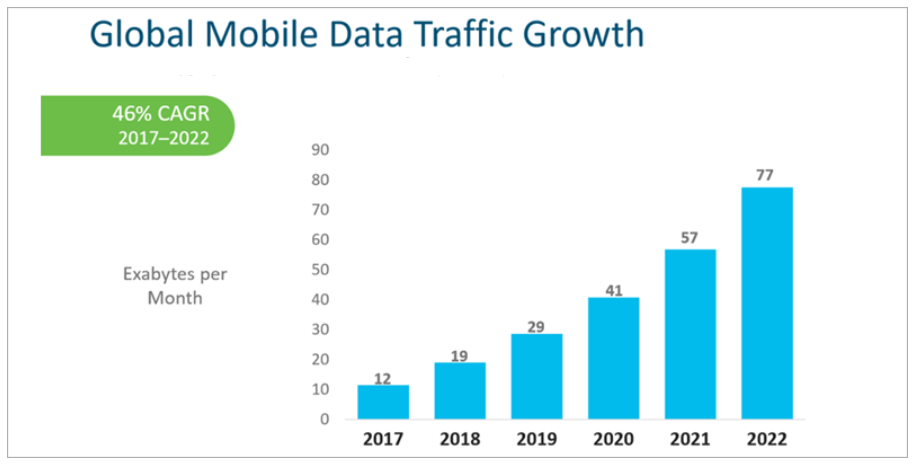
\includegraphics[scale=0.70]{./figuras/data_traffic.png}
    \caption{\small{Gráfica del aumento de tráficos de datos en el mundo expresado en exabytes por mes. Fuente [4].}}
    \label{data_traffic}%
\end{figure}

Aparte de este problema, la comunicación por radiofrecuencia tiene más: \cite{khan}

\begin{itemize}
    \item Interferencia: vivimos rodeados de dispositivos eléctricos que producen ondas electromagnéticas que pueden interferirse entre sí o incluso con señales de dispositivos inalámbricos inhabilitando su comunicación.
    \item Latencia: el principal objetivo de la radiofrecuencia es la baja latencia, pero es cierto que en la realidad siempre surgen problemas de alta latencia.
    \item Seguridad: las ondas electromagnéticas penetran muy fácilmente por las paredes y pueden causar problemas de seguridad en la que personas ajenas puedan atacar tus dispositivos.
    \item Salud: como se ha comentado al inicio del apartado.
\end{itemize}

Por todo esto es importante el desarrollo de otras técnicas entre las que destaca la de comunicación por luz visible debido a sus características de canales sin licencia, alto ancho de banda y bajo consumo, que pueden ayudar a reducir el tráfico de datos y los niveles de exposición a ondas electromagnéticas.

\section{Ventajas y ámbito de aplicación}

En el apartado anterior se ha comentado la problemática del principal sistema de comunicación por lo que es importante ver cuáles serían las ventajas de la comunicación por luz visible respecto a las ondas electromagnéticas.

La comunicación por luz visible ocupa el espectro de frecuencia de 430 THz a 790 THz como se muestra en la figura 1.4. Este método de comunicación no tiene problemas respecto a las interferencias o a la alta latencia ya que posee un gran ancho de banda y presenta inmunidad a las interferencias procedentes de fuente electromagnéticas. Además, su implementación viene ligada al remplazo de las lámparas fluorescentes por diodos led, que además, tienen la capacidad de emitir información. \cite{khan}

\begin{figure}[ht]
    \centering
    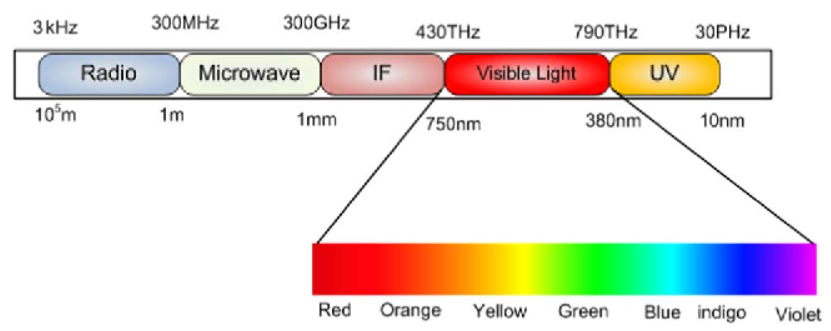
\includegraphics[scale=0.70]{./figuras/espectro.png}
    \caption{\small{Espectro de frecuencia VLC. Fuente [4]}}
    \label{espectro}%
\end{figure}
\newpage
Es importante resaltar las potencialidades de la comunicación por luz visible, por lo que, aunque el proyecto se centre en la comunicación entre vehículos, a continuación, se van a presentar distintas aplicaciones de comunicación por luz visible [4].

\begin{itemize}
    \item Li-Fi: es análogo al Wi-Fi y se describe como un sistema de comunicación inalámbrica de luz visible bidireccional. No tiene problemas de interferencia (por ejemplo, en aviones) y obtiene una velocidad de hasta 10 Gbits/s (250 veces mayor que la banda ancha super rápida).
    \item Comunicación entre vehículos: es la aplicación en la que se va a centrar el proyecto. Permite la comunicación entre vehículos e infraestructura de manera segura previniendo de posibles accidentes y ayudando a un conducción más segura y eficiente debido a la alta velocidad de comunicación.
    \item Comunicación bajo el agua: las ondas electromagnéticas no viajan bien en el agua del mar ya que esta no es buena conductora. Sin embargo, la luz en colores azules y verdes puede ser transmitida íntegramente, lo que puede ser útil en aplicaciones ROUV (\textit{remotely operated underwater vehicle}).
    \item Hospitales: en los hospitales hay áreas sensibles a ondas electromagnéticas en las que no se recomienda su uso. Así que, es importante desarrollar sistemas por luz visible para no causar problemas por radiaciones electromagnéticas.
\end{itemize}

\section{Proyectos relacionados con la comunicación por luz visible entre vehículos}

Es importante tener algunos proyectos y trabajos de referencia para poder saber si lo que 
se está haciendo es correcto o no. Por lo tanto, es imprescindible contar con que estos 
sean accesibles a todo el mundo.

Algunos de estos proyectos para ser tomados de referencia son:

\begin{itemize}
    \item \textit{Visible Light Communication for Cooperative ITS}: este proyecto está 
    desarrollado por National Laboratory of Photonic Networks en Pisa, Italia. Dicho 
    proyecto se encuentra muy bien documentado y se centra en la explicación de la 
    arquitectura de transmisión y recepción, así como de su aplicación en un entorno ITS en 
    el que se está en continua comunicación tanto con otros vehículos como con la 
    infraestructura cercana, además de contemplar su respuesta a las posibles interferencias. \cite{falci}
    \item \textit{Impact of IEEE 802.15.7 Standard on Visible Light Communications Usage in 
    Automotive Aplications}: este proyecto autoriza la licencia de uso a la Universidad de 
    Málaga. Desarrolla la comunicación por luz visible desde un punto de vista más teórico 
    a través del estándar en el que se explican el Dimming, las topologías, la modulación 
    en frecuencia y la estructura de trama. \cite{caile}
\end{itemize}

Por todo esto, en conclusión, se van a tomar como referencia ambos proyectos. Aunque es 
importante destacar que nuestro proyecto diferirá en gran medida con ambos ya que añadirá 
el uso de diferentes esquemas de señalización para transmitir la señal y recibirla además 
del uso de varios sistemas de decisión para regenerar la señal recibida. También es 
importante la diferencia respecto a la herramienta 
de recepción, que en nuestro caso será una matriz de puertas lógicas programables (FPGA) 
así como de su respectiva programación en lenguaje VHDL.
\newpage
\section{Esquemas de señalización}
% Hablar sobre la importancia de los esquemas de señalización y de que son el enfoque principal del TFG.
Un esquema de codificación estandariza la codificación de caracteres mediante la definición de un 
método único para representar los datos de tipo carácter. 

La señal que se desea enviar no tiene por qué ser transmitida literalmente ya que las señales digitales tienen la posibilidad de 
ser codificadas para mejorar, por ejemplo, la detección de la misma en recepción y la probabilidad de corregir errores.

Por tanto, el enfoque principal de este proyecto es desarrollar distintos esquemas de codificación para conocer sus propiedades específicas y
sus ventajas e inconvenientes en las comunicaciones por luz visible. Para implementar dichos esquemas se desarrollará tanto el 
codificador (módulo del transmisor) como el decodificador (módulo del receptor), además de distintos sistemas de decisión para
hacer más robusta la transmisión y disminuir la probabilidad de errores.

Además de implementar distintos esquemas de señalización también se desarrollarán varios
sistemas de decisión para interpretar y regenerar la señal recibida para dotar de mayor
resistencia al ruido disminuyendo los errores.

\section{Estructura del documento}

El desarrollo del proyecto se dividirá en cinco apartados diferenciados.

El primero consiste en explicar la tecnología que se ha empleado para implementar el 
proyecto diferenciando entre la tecnología hardware y software.

El segundo, en comentar en que consiste el sistema de comunicación centrándonos en el 
estándar VLC y en el sistema de partida que se heredó tanto hardware como software.

El tercero será el apartado teórico que desarrollará las bases sobre las 
cuales se ha construido el trabajo describiendo los esquemas de señalización empleados,
así como los sistemas de decisión.

El cuarto es el de implementación en el cual se explicará cómo se ha traducido a la 
realidad todo lo desarrollado en el apartado anterior.

El quinto y último apartado será el apartado de pruebas en el que se muestra el 
funcionamiento de todo lo implementado en una transmisión/recepción de luz real.

\section{Objetivo}
\label{sec:intro:obj}
El objetivo global de este proyecto es la realización de un sistema de comunicación por luz
visible orientado a vehículos a través de una matriz de puertas lógicas programable
(FPGA) que actúa de intermediaria entre el transmisor y el receptor, cumpliendo con el
estándar IEE 802.15.7-218.

Este objetivo se desarrollará implementando varias técnicas de transmisión y recepción siendo estas la implementación de 
diferentes esquemas de codificación de la señal, desarrollando el codificador y el decodificador, y la implementación de distintos sistemas de 
decisión para interpretar la señal recibida antes de decodificarla. 
Además, el sistema deberá tener robustez ante posibles
efectos adversos provocados por las condiciones meteorológicas y un rango de
alcance lo suficientemente alto para cubrir una distancia considerable entre coches.

\chapterend
